\documentclass[10pt,a4paper,titlepage]{jreport} % ドキュメントクラスを1つに統一


\usepackage[top=25truemm,bottom=25truemm,left=20truemm,right=20truemm]{geometry} % 余白設定
\usepackage[dvipdfmx]{graphicx} % 画像の挿入
\usepackage{graphicx}
\usepackage{listings} % コードリスト用
\usepackage{jlisting} % 日本語対応のリスト用
\usepackage{jverb} % 日本語のベタ打ち
\usepackage{booktabs}
\usepackage{pgfplots} % グラフ描画用パッケージ
\pgfplotsset{compat=1.18} % バージョン指定
\usepackage{float}
\parindent = 0pt % 段落の字下げを無効化

\usepackage{titlesec}
\usepackage{etoolbox}
\makeatletter
\patchcmd{\chapter}{\if@openleft\cleardoublepage\else\if@openright\cleardoublepage\else\clearpage\fi\fi}{}{}{}
\makeatother
\lstset{breaklines=true, postbreak=\mbox{$\hookrightarrow$}\space, keepspaces=true, escapeinside={\%*}{*)}}

\titleformat{\chapter}[hang] % 章のフォーマットを変更
  {\normalfont\huge\bfseries} % フォント設定
  {\thechapter} % 番号部分の表示形式
  {1em} % 番号とタイトルの間のスペース
  {} % タイトルの前に入れる内容（ここでは空）
\usepackage{xcolor}
\usepackage{amsmath}
\usepackage{amssymb} % ←これで \mathbb{R} が使える

\lstset{
  language=Matlab,              % 言語はMATLAB
  basicstyle=\ttfamily\small,   % フォントは等幅、サイズ小さめ
  keywordstyle=\color{blue},    % キーワード（function, endとか）を青
  commentstyle=\color{green!50!black}, % コメントを深緑
  stringstyle=\color{red!70!black},    % 文字列（'...'）を赤系
  numbers=left,                 % 行番号を左に表示
  numberstyle=\tiny\color{gray},% 行番号をグレーで小さく
  stepnumber=1,                 % 毎行行番号つける
  numbersep=10pt,               % コードとの間隔
  backgroundcolor=\color{gray!10}, % 背景うっすらグレー
  frame=single,                 % 枠をつける
  rulecolor=\color{black},      % 枠線は黒
  breaklines=true,              % 長い行を折り返す
  breakatwhitespace=false,      % スペースでだけ折り返すか（falseにして自然な折り返し）
  showspaces=false,             % スペースは特別に表示しない
  showstringspaces=false,       % 文字列中のスペースも普通に表示
  tabsize=2                     % タブ幅2
}


\title{最終レポート} % タイトル
\author{
  テーマ：知的システム工学実験演習II C101：統計情報処理 \\
学生番号：242C2016 \\
  氏名：奥村直 \\
  知的システム工学科システム制御コース
} % 著者
\date{\today} % 日付

\begin{document}

\maketitle

\chapter{第1週}

\section{実験目的}

第1週では、基本的な確率統計の知識と仮説検定について学び、演習を通して
理解を深めることを目的とする。

\section{原理・前提知識（統計解析の基礎）：第1週のまとめ}

\textbf{確率変数} ・・・ 確率的に値が決まる変数 \\
\textbf{事象・標本空間} ・・・ 試行によって起こり得る結果のことを事象と
いい、起こり得る結果の全体をその試行の標本空間という。\\
\textbf{確率分布} ・・・ 確率変数の値に対応し、その値が起きる（得られる）
確率をまとめたもの \\

\textbf{平均} ： $\mu = \sum_{i}^{} p_{i}x_{i} = p_{1}x_{1} + p_{2}x_{2} + ～ + p_{n}x_{n}$ \\
\textbf{分散} ： $\sigma^2 = \sum_{i}^{} p_{i}(x_{i} - \mu)^2 = p_{1}(x_{1} - \mu)^2 + p_{2}(x_{2} - \mu)^2 + ～ + p_{n}(x_{n} - \mu)^2$ \\
\textbf{標準偏差} ： $\sqrt{\sigma^2}$\\

\textbf{二項分布} ・・・ 二項分布とは2つの結果のみの試行をn回繰り返したときに、ある結果がk回起こる確率に従う確率分布。\\
\textbf{正規分布} ・・・ 連続的な確率変数を考察するときに用いられる確率密度関数\\

\textbf{正規分布の確率密度関数} ： $p(x) = \frac{1}{\sqrt{2\pi\sigma^2}} exp\left[-\frac{(x-\mu)^2}{2\sigma^2}\right] $\\

\textbf{仮説検定} ・・・ 仮説では、設定されたある確率に従い事象が起きるはずである。
しかし、実際に起きた事象を観測すると仮説が疑わしく感じることもある。
仮説検定は、仮説を棄却するか採択するかを統計学的に判断する手法である。

\textbf{有意水準} ・・・ 一般的には、帰無仮説 $H$ が正しい場合でも誤って棄却してしまうことがある。仮説検定では、この誤りを第1種の過誤と呼び、
第1種の過誤を犯す確率を有意水準と呼ぶ。\\

有意水準を単に低くして検定すると、棄却するべき帰無仮説を見逃してしまうことがあり、安易に有意水準は低くすることができない。
また、この帰無仮説を見逃してしまうことを第2種の過誤という。

\section{レポート課題１}

表が0.6の確率で出るイカサマコインを購入した。購入したコインが
実際に規格通りであることを確認するため、100回コイントスする試行
により仮説検定を行う。（表の出る確率が0.6であることを確かめたい）
ここで帰無仮説を $H_0$ 「コインが規格通り製造されている」とする。

\subsection{課題（i）}

演習１を参考に、表が0.6の確率で出るコインを100回コイントスしたときの
二項分布をセット数500で確認し、頻度分布を示しなさい。

\subsubsection{原理}

二項分布で、頻度分布を調べるとその頻度の事象が起こる確率に相当する回数
付近に結果が最も集まるようになる。今回は表が出た回数の頻度分布について
調べているため、表の出る確率に相当する頻度付近に集中している。

\subsubsection{ソースコード}

\begin{lstlisting}[caption=kadai1]
n = 100;              % コイントス回数
numof_set = 500;      % セット数
fre = zeros(n + 1, 1);

x = 0:n;

p_d = [0, 1];         % 裏=0, 表=1
w = [0.4, 0.6];       % 表が出る確率0.6

for i = 1:numof_set
    s_d = datasample(p_d, n, 'Weights', w);
    numof_heads = sum(s_d);
    fre(numof_heads + 1) = fre(numof_heads + 1) + 1;
end

bar(x, fre);
title('表が出る確率0.6のコインを100回投げたときの二項分布');
xlabel('表が出た回数');
ylabel('頻度（セット数）');
\end{lstlisting}

\subsubsection{実験結果}

上記ソースコードの実行結果として下（図1.1: kadai1）に示すヒストグラムが得られた

\begin{figure}[H]
  \centering
  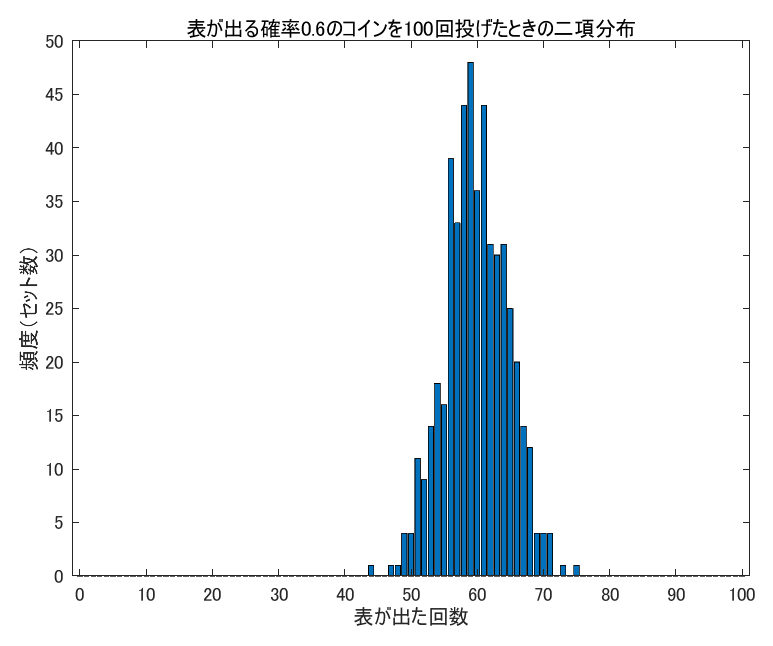
\includegraphics[width=0.8\linewidth]{kadai1.eps}
  \caption{kadai1i}
  \label{fig:sample}
\end{figure}

\subsubsection{考察}

課題（i）では、表が出る確率が0.6であるコインを100回投げる試行を500セット行い、
表が出た回数の頻度分布を確認した。得られた頻度分布は、表の出る回数が60回付近
を中心とした釣鐘型の分布となり、二項分布B(100,0.6) の理論的な形状とよく一致
していることが確認できた。

\subsection{課題（ii）}

有意水準 5\% で検定する際、100回中何回表が出ると仮説が棄却されるか、
その範囲を計算し、課題（i）で得られた頻度分布にその範囲を示しなさい。

\subsubsection{原理}

否定されることを期待してたてる（無に帰すことを目的とした）仮説を\textbf{帰無仮説 $H_0$} といい、
帰無仮説に対立する仮説を\textbf{対立仮説 $H_1$} という。\\
また、棄却されることが期待されている帰無仮説 $H_0$ が正しいのにも関わらず棄却して
しまう間違いを第1種の過誤、本来は棄却すべき帰無仮説を正しいと判定してしまうことを第2種
の過誤と呼ぶ。この課題（ii）では、有意水準5\%で検定する際、100回中何回表が出たときに棄却されるか、
その範囲を求める。表が出た回数を $x$ 、その事象が発生する確率を $p$ 、
試行回数を $n$ とすると、ここでの標準正規分布は

\begin{equation}
Z = \frac{x - \mu}{\sigma}
\end{equation}

より、

\begin{equation}
Z = \frac{x - np}{\sqrt{np(1-p)}}
\end{equation}

と表現できる。

\subsubsection{ソースコード}

\begin{lstlisting}
p = 0.6; %表が出る確率
n = 100;              % コイントス回数
numof_set = 500;      % セット数
fre = zeros(n + 1, 1);

x = 0:n;

p_d = [0, 1];         % 裏=0, 表=1
w = [0.4, 0.6];       % 表が出る確率0.6

for i = 1:numof_set
    s_d = datasample(p_d, n, 'Weights', w);
    numof_heads = sum(s_d);
    fre(numof_heads + 1) = fre(numof_heads + 1) + 1;
end

bar(x, fre);
title('表が出る確率0.6のコインを100回投げたときの二項分布');
xlabel('表が出た回数');
ylabel('頻度（セット数）');
np = n * p; 
npq = n * p * (1 - p); %平均、分散の定義
variant1 = -1.96 * sqrt(npq) + np; %棄却域
variant2 = 1.96 * sqrt(npq) + np; %棄却域の算出
xline(variant1,'-','棄却域','Color','r'); %棄却域を赤の実線で書き込む
xline(variant2,'-','棄却域','Color','r'); %棄却域を赤の実線で書き込む
legend('頻度分布',...
 strcat('棄却域：限界値:',num2str(variant1)),...
 strcat('棄却域：限界値:',num2str(variant2))); %説明の追加
title(strcat('レポート課題 1 課題(ii)')); %タイトル表示
\end{lstlisting}

\subsubsection{実験結果}

\begin{figure}[H]
  \centering
  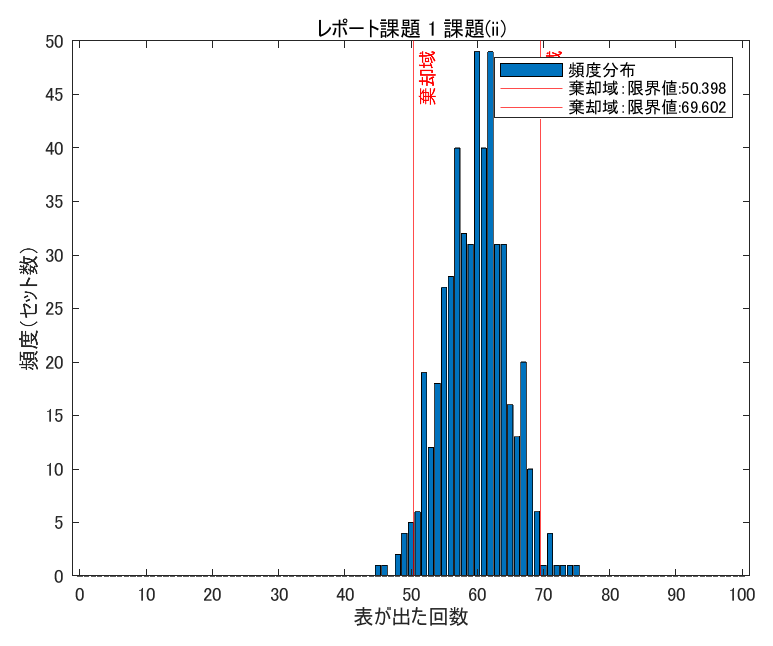
\includegraphics[width=0.8\linewidth]{kadai1ii.eps}
  \caption{kadai1ii}
  \label{fig:sample2}
\end{figure}

\subsubsection{考察}

図1.2: kadai1iiを見ると、0回から約50回または7約70回から約100回表が出ると
この仮説は棄却されるということが分かった。

\subsection{課題（iii）}

（i）の状況では仮説を棄却しないことが正しいが500セット中で何回仮説を棄却
してしまったか確認し、仮説検定において有意水準によって第１種の過誤を侵す
確率を制御できていることを確認しなさい。

\subsubsection{原理}

課題（ii）で説明していた、第1種の過誤が発生する確率を \textbf{有意水準} という。
ここでは仮説を棄却しないことが正しいため、第1種の過誤（正しいにも関わらず仮説が棄却されること）
の可能性があるセットは棄却域に分布しているセットである。そのセットを数えて、数えたセットが全体の
セットの数に対して何割かを算出すればよい。
算出した結果が0.05付近であれば、制御できていると考えてよい。

\subsubsection{結果・考察}

図1.2を見て、棄却域にあるセットを目視で計上した。すると22セットあると
分かったので原理で言及した割合を算出する。有意水準 $\phi$ は、

\begin{equation}
\phi = \frac{22}{500} = 0.044...[\%]
\end{equation}

結果より、計算結果が有意水準 $5\%$ 付近であるから、仮説検定において有意水準によって
第１種の過誤を侵す確率を制御できていることを確認できた。


\chapter{第2週}

\section{実験目的}

第2週では、代表的な乱択アルゴリズムであるモンテカルロ法を学んで乱択
アルゴリズムについての理解を深める。

\section{原理・前提知識（モンテカルロ法）：第2週のまとめ}

\textbf{乱択アルゴリズム}

乱択アルゴリズムとは、無作為抽出を含むアルゴリズムのことである。基本的な
考え方は、解析的には解くことができなかったり、解くことが（計算量的に）非常に
難しい問題に乱択を導入することで確定的な解を得ることを諦め、確率的な解を得る
方法である。確定的な解を得ることを諦める代わりに現実的な計算時間で確率的な解を
得ようという考え方である。また、乱択アルゴリズムに共通する特徴としては、
ある精度を保証するために必要な乱択の回数は、問題の複雑さや難しさに依存せず
に決まることにある。また、アルゴリズムの実装、並列化も容易である。
\\
決定論的な問題への簡単な適応例として円周率 $\pi$ をモンテカルロ法で
求めることを考えよう。 $x_i \in [0 1], y_i \in [0 1]$ をそれぞれ
一様乱数とし、N組のサンプルに対して、

\begin{equation}
{x_i}^2 + {y_i}^2 \leqq 1
\end{equation}

を満たす組の数をSとする。与式を満たす確率は、正方形と $\frac{1}{4}$ 円の
面積比 $\frac{\pi}{4}$ に比例するはずであるから、円周率 $\pi$ の近似値は

\begin{equation}
\pi \approx \frac{4S}{N}
\end{equation}

と求められる。\\ 

\textbf{定理１：大数の弱法則}

確率変数 $X_1, X_2, ..., X_N$ が独立であって、それらの平均が $E(X_k) = \mu (\forall k)$ 、かつ、一定の
定数 $\sigma$ に対して $V(X_k) \leqq \sigma^2(\forall k)$ であるならば、Nが十分大きくなると
 $\widetilde{X} = \frac{1}{N} \sum_{k = 1}^{N} X_k$
は $\mu$ に確率収束する。つまり、任意に与えられる整数 $\epsilon > 0$ に対して

\begin{equation}
\lim_{N \to \infty} P(\left\lvert \widetilde{X} - \mu \right\rvert < \epsilon) = 1  
\end{equation}

この定理１によって、試行回数を大きくすれば近似値が真値に近づくことが保障される。
ただし、試行回数を増やすほど、近似値が単調に真値に近づくとは述べていない。さらに、
近似の制度を見積もるためには次の定理が重要である。

\textbf{定理２：中心極限定理}

確率変数 $X_1, ..., X_N$ が平均 $\mu$ 、分散 $\sigma^2$ の独立同分布の確率変数
とする。nが十分大きければ $\widetilde{X} = \frac{1}{N}\sum_{k = 1}^{N} X_k$ は
平均 $\mu$ 、分散 $\frac{\sigma^2}{N}$ の正規分布に従う。
　この中心極限定理を用いて近似制度を見積もってみる。確率変数 $X_k$ をk回目の試行で
条件を満たす場合に1、満たさない場合に0をとるものとする。このようにすると、 $\widetilde{X}$ は
相対度数 $\frac{S}{N}$ に等しい。また、 $X_k$ の平均 $E(X_k)$ と
分散 $V(X_k)$ は、真の確率を $I (= \frac{\pi}{4})$ とすると、

\begin{equation}
E(X_k) = I
\end{equation}

\begin{equation}
V(X_k) = I(1 - I)^2 + (1 - I)(0 - I)^2 = I(1 - I)
\end{equation}

である。これらと中心極限定理より $\widetilde{X}$ の平均 $E(\widetilde{X})$ 
と分散 $V(\widetilde{X})$ は

\begin{equation}
E(\widetilde{X}) = I
\end{equation}

\begin{equation}
V(\widetilde{X}) = \frac{1}{N}I(1 - I)
\end{equation}

となる。

円周率を求めるこの例題の場合、信頼度99\%でIの真の値は

\begin{equation}
\frac{S}{N} \pm \frac{2.5758}{4}\sqrt{\frac{\pi(4 - \pi)}{N}}
\end{equation}

の区間に含まれる。およそ10000回の試行で信頼区間は約 $\pm 0.01$ となる。
また、信頼区間の幅を $\frac{1}{10}$ 倍にするためには、試行回数 $N$ を100倍
にする必要があることが分かる。

\section{レポート課題２}
\subsection{課題（i）}

セットあたりの試行回数を $10^2, 10^3, 10^4$ と増加させて【演習６】と同様に
グラフにプロットして、平均、分散も確認して「大数の法則」、「中心極限定理」
について考察しなさい。

\subsubsection{原理}

原理については節「原理・前提知識（モンテカルロ法）：第2週のまとめ」の大数の法則と
中心極限定理を参照。

\subsubsection{ソースコード}

\begin{lstlisting}[caption=kadai2i]
clear; close all; %初期化
N=2:4; %試行回数 10^2~10^4
numof_set=100;
step=5^(N(1)-1)/(10^N(1));
min_x=pi-(0.5+step*0.5); %下限
max_x=pi+(0.5+step*0.5); %上限
Region=[min_x,max_x;0,numof_set]; %ヒストグラム描画の領域設定
title('中心極限定理の確認');
for e=1:length(N)
subplot(1,length(N),e); %同一ウィンドウにグラフを複数描画
plot([pi,pi],[0,numof_set]); %y=π の線を描画
legend('真の円周率');
xlabel({'推定された円周率',sprintf('(試行回数:%d)',10^N(e))});
ylabel('頻度');
hold on;
end
i_est=zeros(length(N),numof_set); %推定結果格納用
for e=1:length(N) %1セットあたりの試行回数が同じセットをまとめて実行
numof_try=10^N(e);
%%%%%%%ベクトル演算%%%%%%%%
x=rand(numof_try,numof_set); %乱択で選ばれた x 座標(numof_try×numof_set の配列)
y=rand(numof_try,numof_set); %乱択で選ばれた y 座標(numof_try×numof_set の配列)
cnt=sum(((x.^2+y.^2)<=1),1); %x^2+y^2<1 が真(%t)となった要素数
i_est(e,:)=cnt/numof_try; %π/4 の推定結果を格納
%%%%%%%%%%%%%%%%%%%%%%%%%%%
fprintf('-----------------------------\n');
fprintf('試行回数: %d\n',10^N(e));
fprintf('平均 : %.5f\n',mean(i_est(e,:)*4)); %π(=4I)の推定値について
fprintf('標準偏差: %.8f\n',std(i_est(e,:)*4)); %統計量を計算、表示
subplot(1,length(N),e);
histogram(i_est(e,:)*4,min_x:step:max_x);
end
\end{lstlisting}

\subsubsection{実験結果}

\begin{figure}[htbp]
  \centering
  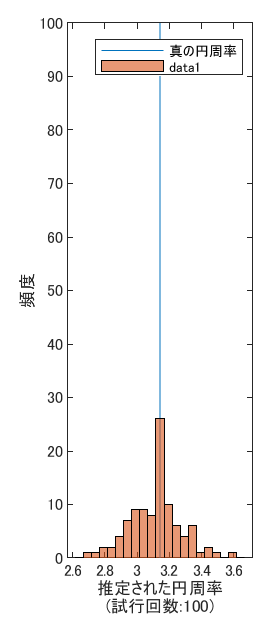
\includegraphics[
    width=0.8\linewidth,
    height=0.75\textheight,
    keepaspectratio
  ]{kadai2i1.eps}
  \caption{kadai2i1}
  \label{fig:sample3}
\end{figure}

\clearpage

\begin{figure}[htbp]
  \centering
  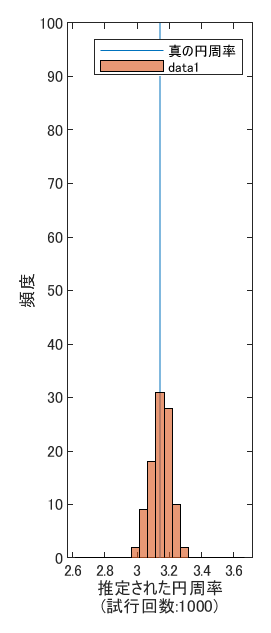
\includegraphics[
    width=0.8\linewidth,
    height=0.75\textheight,
    keepaspectratio
  ]{kadai2i2.eps}
  \caption{kadai2i2}
  \label{fig:sample4}
\end{figure}

\clearpage

\begin{figure}[htbp]
  \centering
  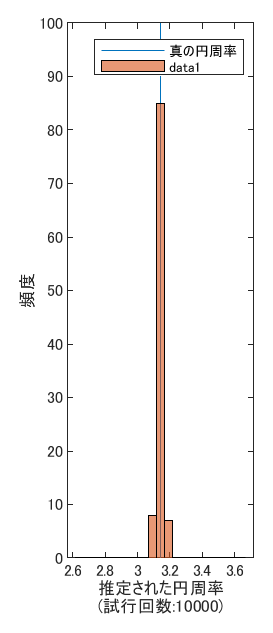
\includegraphics[
    width=0.8\linewidth,
    height=0.75\textheight,
    keepaspectratio
  ]{kadai2i3.eps}
  \caption{kadai12i3}
  \label{fig:sample5}
\end{figure}

\clearpage

\begin{lstlisting}[caption=kadai2i]
-----------------------------
試行回数: 100
平均 : 3.11440
標準偏差: 0.15979987
-----------------------------
試行回数: 1000
平均 : 3.15028
標準偏差: 0.06354956
-----------------------------
試行回数: 10000
平均 : 3.14030
標準偏差: 0.01696000
\end{lstlisting}

\subsubsection{考察}

セットあたりの試行回数を $10^2, 10^3, 10^4$ と変化させ、それぞれについて推定された円周率の分布、
平均および分散を確認した。まず平均値に注目すると、試行回数が $10^2$ の場合には平均値は
真の円周率 $\pi$ からややずれているが、 $10^3, 10^4$ と試行回数を増加させるにつれて、平均値は真の値
に近づいていることが分かる。これは、試行回数が十分に大きくなると標本平均が期待値
に収束するという 大数の法則 を反映した結果である。次に分散を見ると、
試行回数の増加に伴って値が大きく減少しており、推定値のばらつきが小さくなっていることが確認できる。
実際に、標準偏差はおおよそ試行回数の平方根に反比例して減少しており、
試行回数が増えるほど推定精度が向上している。
また、ヒストグラムの形状に着目すると、試行回数が少ない $10^2$ では分布がやや歪んでいるのに対し、
$10^3, 10^4$では平均値の周りに左右対称な釣鐘型の分布に近づいている。
これは、各試行結果の分布に関わらず、標本平均の分布が正規分布に近づくという 中心極限定理 を示している。

\subsection{課題（ii-a）}

$10^2, 10^3, 10^4$ の各試行回数の１セットについて、それぞれ、(2.8)式
にて示された99\% 信頼区間に真の確率 $I(=\frac{\pi}{4})$ が得られている
セットの総数を求めるコマンドをプログラムに追加し、得られた結果から信頼区間
について考察しなさい。

\subsection{課題（ii-b）}

同様に、95\% 信頼区間についても確認しなさい。

\subsubsection{ソースコード}

\end{document}
